\documentclass[12pt]{article}

\usepackage{siunitx}
\usepackage{fouriernc}
\usepackage{color}
\usepackage{amsmath,amssymb}
\usepackage{natbib}
\usepackage{bm,bbm}
\usepackage{enumitem}
\usepackage{graphicx}
\graphicspath{{./Figures/}}

\usepackage[indent=1cm]{parskip}

\title{Research Proposal}

\begin{document}
\maketitle
	
We already have purely empirical results about the confidence region of points in the $H\times C$ plane under white noise.
In this work, we propose advancing such a knowledge by using a general model for discrete distributions.
The work by \citet{OrdinalPatternProbabilities} is among the few that study theoretical (distributional) properties of these points; the article proves consistency and asymptotic normality of estimators.

\section{Introduction}

Let ${\mathcal X} \equiv \{x_t\}_{t=1}^{T}$ be a real-valued time series of length $T$, without ties. 
As stated by \citet{PermutationEntropyBandtPompe} in their seminal work:  
\begin{quote}
	``If the $\{x_t\}_{t=1}^{T}$ attain infinitely many values, it is common to replace them by a symbol sequence 
	$\Pi \equiv \{\pi_j\}$ with finitely many symbols, and calculate source entropy from it".
\end{quote}
Also, as stressed by these authors, 
\begin{quote}
	``The corresponding symbol sequence must come 
	naturally from the $\{x_t\}_{t=1}^{T}$ without former model assumptions".
\end{quote}

Let ${\mathbbm A}_{D}$ (with $D \geq 2$ and $D \in {\mathbbm N}$) be the symmetric group of order $D!$ formed by all 
possible permutation of order $D$, and the symbol component vector 
${\bm \pi}^{(D)} = (\pi_1, \pi_2, \dots, \pi_D)$ so every element ${\bm \pi}^{(D)}$ is unique 
($\pi_j \neq \pi_k~\forall~j \neq k$). 
Consider for the time series ${\mathcal X} \equiv \{x_t\}_{t=1}^{T}$ its time delay embedding representation,
with embedding dimension $D \geq 2$ ($D \in {\mathbbm N}$) and time delay $\tau \geq 1$ ($\tau \in {\mathbbm N}$, also called ``embedding time''):
\begin{equation} 
	{\mathbf X}^{(D,\tau)}_t =( x_t,x_{t+\tau},\dots,x_{t+(D-1)\tau} ) ,
	\label{eq:time-delay}
\end{equation} 
for $t = 1,2,\dots,N$ with $N = T-(D-1) \tau$.
Then, the vector ${\mathbf X}^{(D,\tau)}_t$ can be mapped to a symbol ${\bm \pi}^{(D)} \in {\mathbbm A}_{D}$. 
This mapping should be defined in a way that preserves the desired relation between the elements 
$x_t  \in {\mathbf X}^{(D,\tau)}_t$, and all $t \in T$ that share this pattern (also called ``motif'') are mapped to the same 
${\bm \pi}^{(D)}$. 
The two most frequent ways to define the mapping ${\mathbf X}^{(D,\tau)} \mapsto {\bm \pi}^{(D)}$ are:  
\begin{enumerate}[label=\alph*)]
	\item ordering the ranks of $x_t \in {\mathbf X}^{(D,\tau)}$ in chronological order 
	(\textit{Rank Permutation}) or,
	\item ordering the time indexes of $x_t \in {\mathbf X}^{(D,\tau)}$  
	(\textit{Chronological Index Permutation}).
\end{enumerate}
See details in the work by \citet{BPRepeatedValuesChaos}.
Without loss of generality, in the following, we will use the latter.

Consider, for instance, the time series $\mathcal X = (2.8, 2.2, 4.2, 5.8, 5.2, 5.5, 3.3, 4.7, 2.2, 1.5)$ depicted in Fig.~\ref{Fig:IntroBP} as a light blue line.
Assume we are using patterns of length $D=5$ with a unitary time lag $\tau=1$.
The code associated to $\mathbf X_{3}^{(5,1)}=(x_3,\dots,x_7)=(4.2, 5.8, 5.2, 5.5, 3.3)$, shown in red, is formed by the indexes in $\bm\pi^{(5)}=(1,2,3,4,5)$ which sort the elements of $\mathbf X_{3}^{(5,1)}$ in increasing order: $51342$.
With this, $\widetilde{\pi}^{(5)} = 51342$, and we increase the counting related to this motif in the histogram of all possible patterns of size $D=5$.

The green line in Fig.~\ref{Fig:IntroBP} illustrates $\mathbf X_{1}^{(5,2)}$, i.e. the sequence of length $D=5$ starting at $x_1$ with lag $\tau=2$.
In this case, $\mathbf X_{1}^{(5,2)}= (2.8, 4.2, 5.2, 3.3, 2.2)$, and the corresponding motif is $\widetilde{\pi}^{(5)}=51423$.

\begin{figure}[hbt]
	\centering
	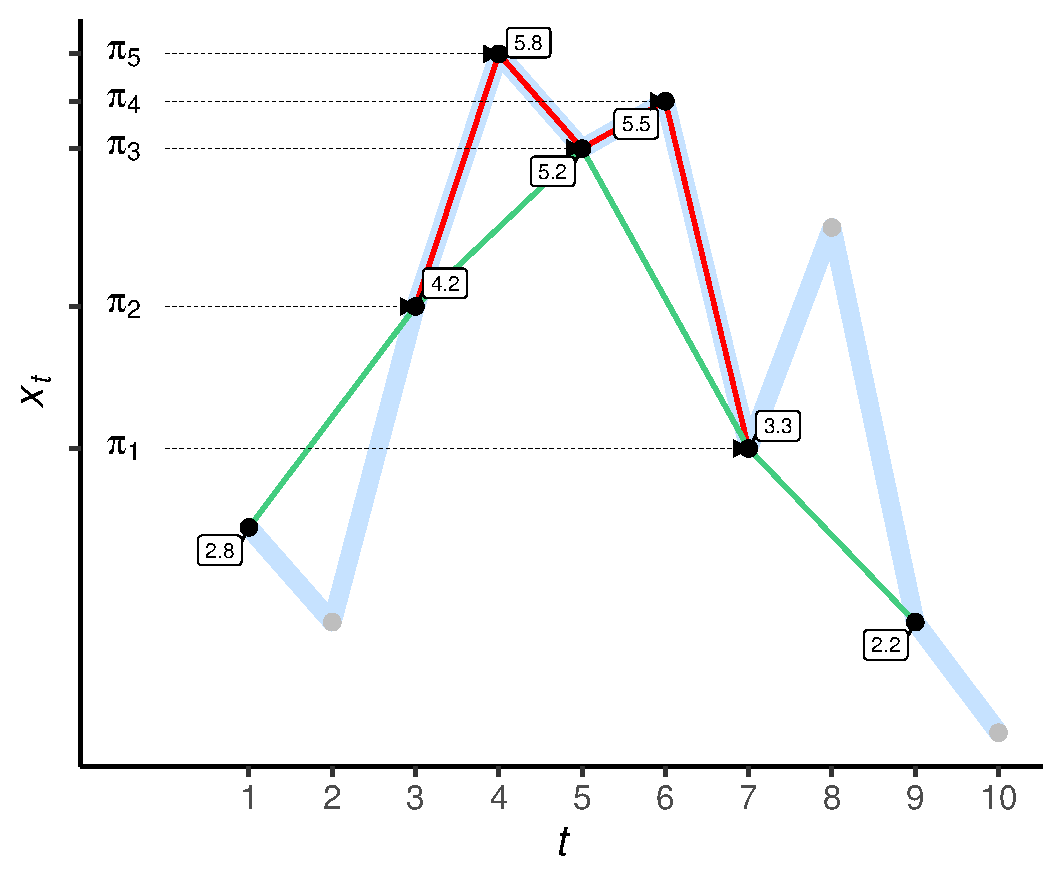
\includegraphics[width=.7\linewidth]{IntroBP}
	\caption{Illustration of the Bandt and Pompe coding}
	\label{Fig:IntroBP}
\end{figure}

After computing all the symbols, one obtains the histogram of proportions $\bm h = (h(j))_{1\leq j\leq D!}$.
Such histogram estimates the (unknown, in general) probability distribution function of these patterns.
The next step into the characterization of the time series is computing descriptors from this histogram.

The first descriptor is a measure of the disorder of the system.
The most frequently used feature for this is the Normalized Shannon entropy, defined as
\begin{equation}
	H(\bm h) = -\frac{1}{\log D!} \sum_{j=1}^{D!} h(j) \log h(j),
\end{equation}
with the convention that terms in the summation for which $h(j)=0$ are null.
This quantity is bounded in the unit interval. 
It is zero when $h(j)=1$ for some $j$ (and, thus, all other bins are zero), and one when $h(j)=1/D!$ for every $j$ (the uniform probability distribution function).

Although very expressive, the Normalized Shannon Entropy is not able to describe all possible underlying dynamics.
In particular, for intermediate values of $H$, there is a wide variety of situations worth characterizing.
To this aim, \citet{LopezRuiz1995} proposed using the disequilibrium  $Q$, a measure of how far $\bm h$ is from an equilibrium or non-informative distribution.
They employed the Euclidean distance between $\bm h$ and the uniform probability distribution function.

We opt for the Jensen-Shannon distance to the uniform distribution $\bm{u} = \big(\frac{1}{D!}, \dots, \frac{1}{D!}\big)$, as it is a measure of how similar the underlying dynamics is to a non-informative process.
It is calculated as:
\begin{equation}
	Q'(\bm{h}, \bm{u}) = \sum_{\ell=1}^{D!} \Big(h_\ell \log\frac{h_\ell}{u_\ell} +
	u_\ell \log\frac{u_\ell}{h_\ell}
	\Big).
\end{equation}
This quantity is also called ``disequilibrium.''
The normalized disequilibrium is $ Q=Q'/\max\{Q'\}$.

With this, they proposed $C=HQ$ as a measure of the Statistical Complexity of the underlying dynamics.
A time series can then be mapped into a point in the $H\times C$ plane.

The Entropy-Complexity plane is the set of all possible points $(h,c)$ that can be produced by arbitrary time series analyzed with embedding dimension $D$ that are mapped on histograms of $D!$ bins.
The time delay is irrelevant, and we consider infinitely long series.

Let us consider two extreme cases:
\begin{enumerate}[label=Case~\Roman*., align=left, leftmargin=*]
	\item 	Strictly monotonically increasing or decreasing series produce a single pattern, so the other $D!-1$ bins of the histogram are zero. 
	The entropy is zero, and the distance to the uniform distribution is maximal. 
	Therefore, the complexity is zero, and such series are mapped onto the point $(0,0)$.
	\item 	White noise produces a histogram of equal proportions $1/D!$ and maximal entropy. 
	The distance to the equilibrium distribution is zero. 
	Thus, such series are mapped onto the point $(1,0)$.
\end{enumerate}

\citet{SomeFeaturesoftheLMCStatisticalComplexity} proved that, for a fixed value of entropy, there are two extreme values of complexity.
\citet{martin2006generalized}, using geometrical arguments on the space of configurations, found expressions for such boundaries.
The lower boundary $C_{\min}$ is smooth, while the upper $C_{\max}$ is defined by $D!-1$ pieces.
The upper boundary converges to a smooth curve when $D\to\infty$.


Fig.~\ref{fig:Boundaries} shows the boundaries of the $H\times C$ plane for the embedding dimensions $D=3$ (red) $D=4$ (green), and $D=5$ (blue).
The inset plot highlights the fine structure of the upper boundary inside the rectangle.
The jagged structure of $C_{\max}$ increases the difficulty of finding distributions for the points in the $H\times C$ plane.

\begin{figure}[hbt]
	\centering
	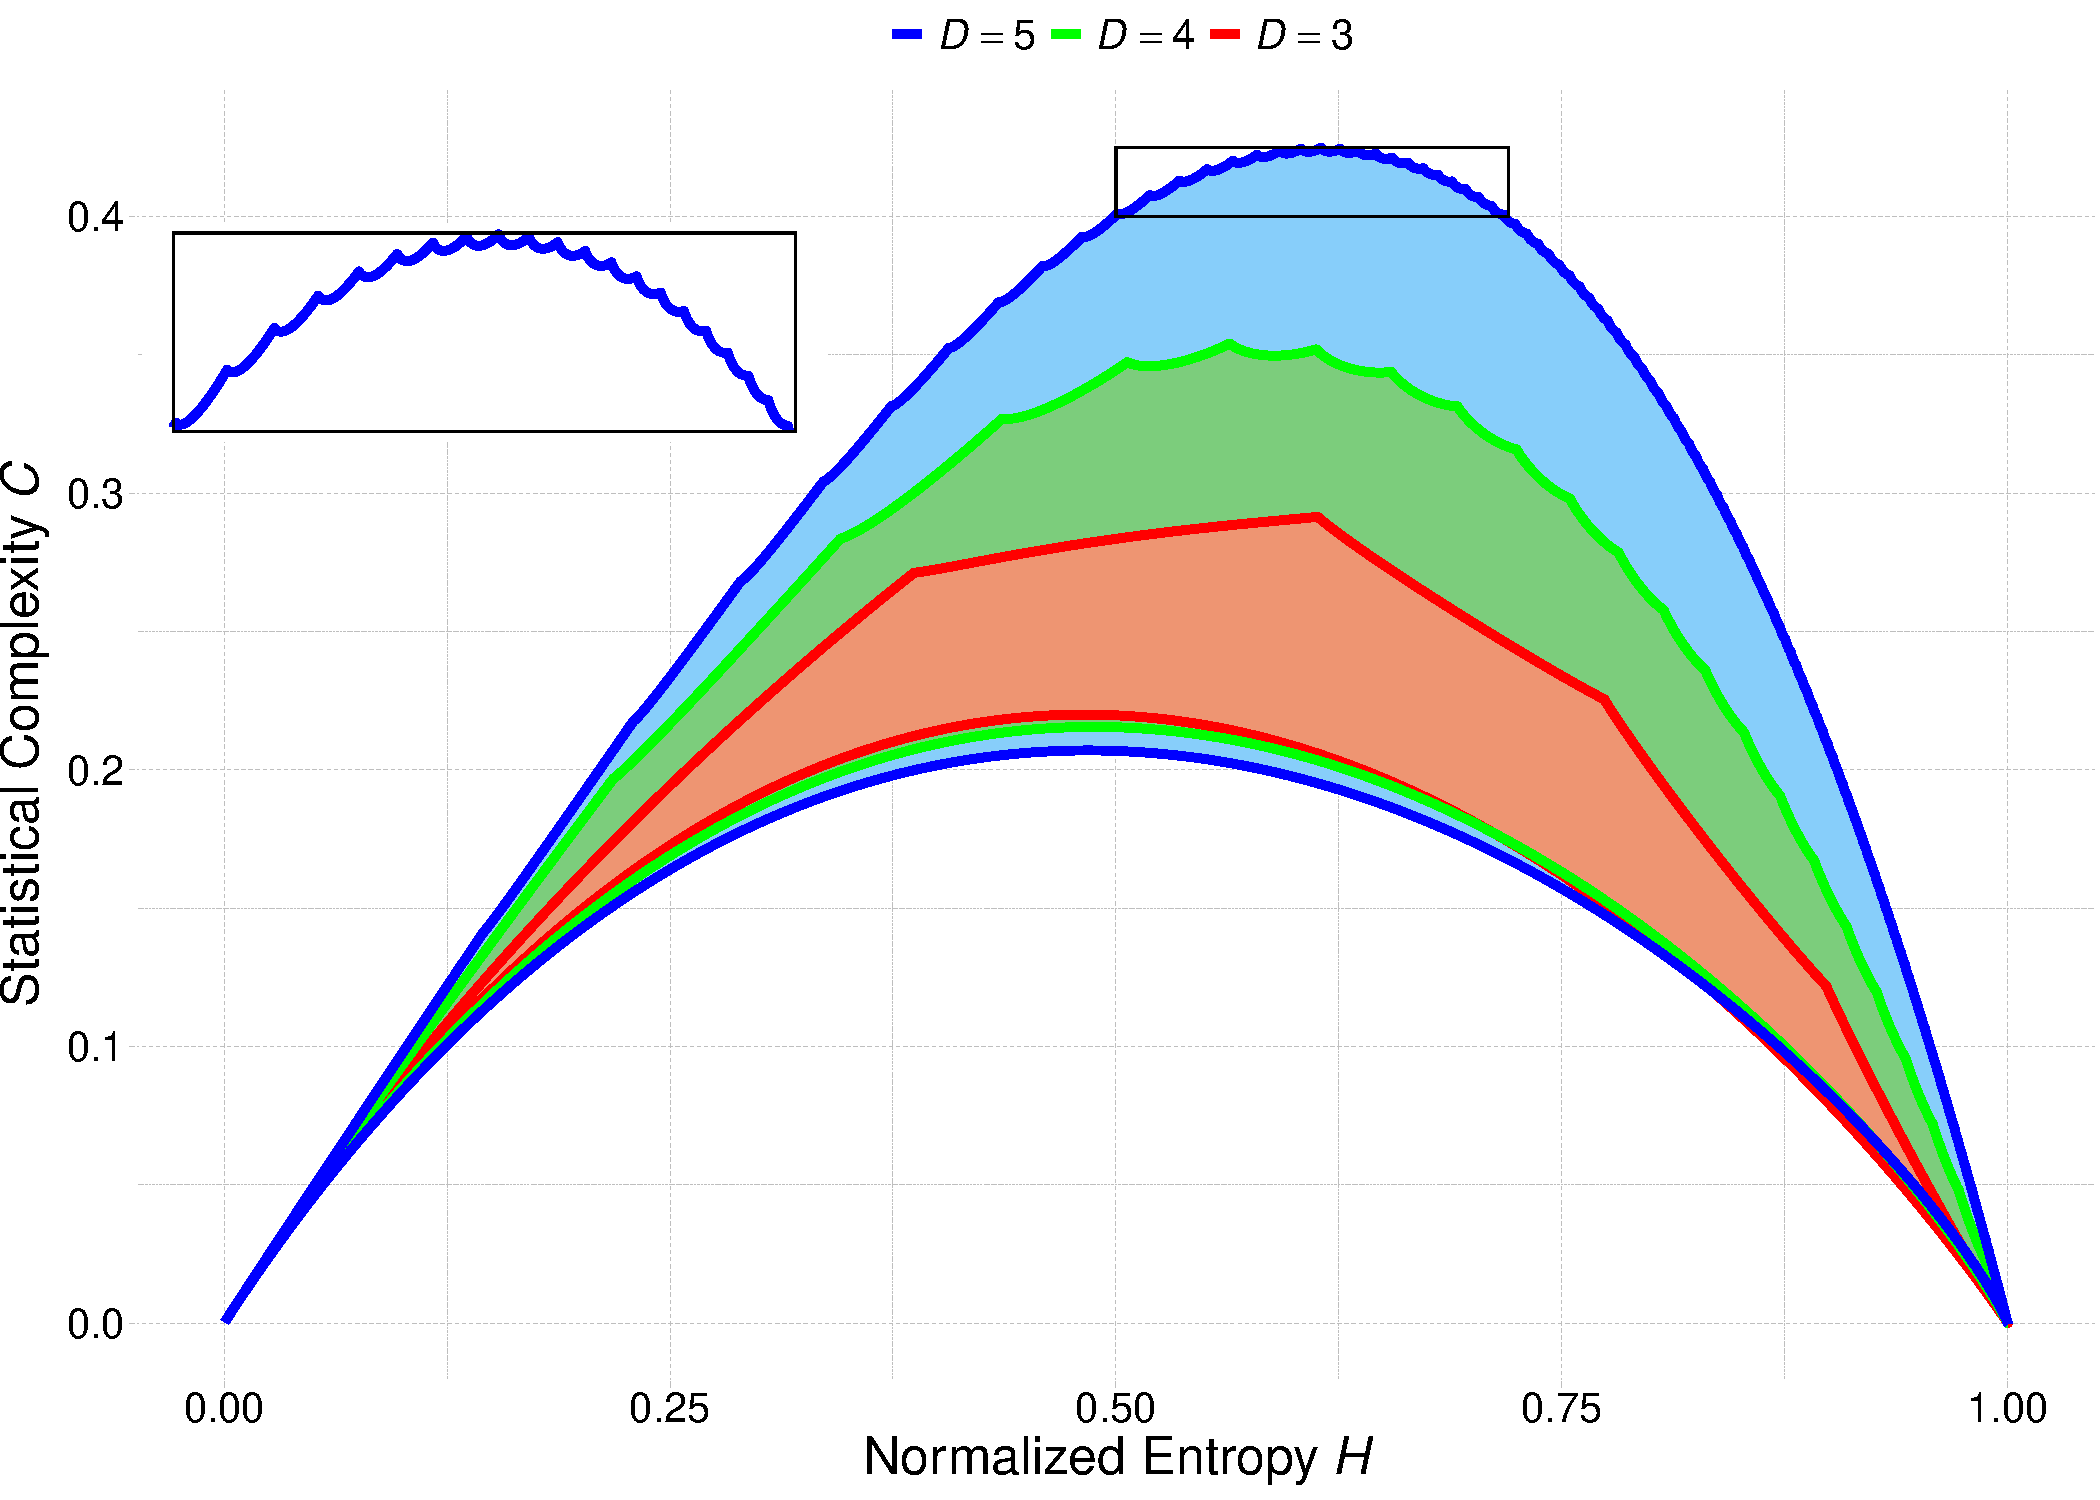
\includegraphics[width=.7\linewidth]{Figures/BoundariesPlot}
	\caption{Boundaries of the $H\times C$ plane for dimension embeddings $D=3,4,5$.}\label{fig:Boundaries}
\end{figure}

Fig.~\ref{fig:RightMostCorner} shows the rightmost lower corner of the $H\times C$ plane, emphasizing the location of the white ($k=0$), $k=1/2$, and pink ($k=1$) noises.

\begin{figure}[hbt]
	\centering
	\includegraphics[width=\linewidth]{RightMostCorner}
	\caption{Representations of white noise, $f^{-1/2}$, and $f^{-1}$ noise in the $H \times C$ plane  for dimension embedding $D = 6$, time delay $\tau = 1$, and sequence length $T = \num[scientific-notation=true]{e4}$.}
	\label{fig:RightMostCorner}
\end{figure}

Due to the infinitude of white noise sequences, although these sequences have the characteristic of presenting high values of entropy and low statistical complexity, their points will not necessarily be located in $(1, 0)$, but in a surrounding region.
In a previous work, we assessed pure randomness by analyzing the empirical distribution of the points produced by true random sequences of finite size and obtaining regions of confidence in the $H \times C$ plane.

In this work, we will use a model to achieve more general results.

\section{The Discretised Beta Distribution}

\citet{ANewVersatileDiscreteDistribution} proposes a flexible discrete model, the ``discretised Beta'' law.
The probability function of such a random variable is
\begin{equation}
\Pr(X  = x \mid \alpha, \beta, n_{\text{top}}, \zeta) = h(x) \exp\big\{ \alpha T_1(x) + \beta T_2(x) - A(\alpha, \beta) \big\},
\label{Eq:ProbdbExponential}
\end{equation}
where $\zeta=\text{TRUE}$ denotes that the support starts in zero ($n_{\text{bot}}=0$), otherwise it starts in one ($n_{\text{bot}}=1$), and
\begin{align}
x &\in \{n_{\text{bot}}, n_{\text{bot}}+1, \dots, n_{\text{top}}\},\\
h(x) & =\frac{(n_{\text{top}} - n_{\text{bot}}+2)^2}{
(x-n_{\text{bot}}+1)	(n_{\text{top}}-x+1)	},\\
T_1(x) &= \log\frac{x-n_{\text{bot}}+1}{n_{\text{top}}-n_{\text{bot}}+2}, \\
T_2(x) &= \log\frac{n_{\text{top}}-x+1}{n_{\text{top}}-n_{\text{bot}}+2}, \\
\intertext{and}
A(\alpha,\beta) &= \log \bigg(
\sum_{i=n_{\text{bot}}}^{n_{\text{top}}} h(i) \exp\big\{ \alpha T_1(i) + \beta T_2(i)\big\}
\bigg).
\end{align}
This definition yields a model that belongs to the exponential family for any $\alpha,\beta\in\mathbbm R$.
Denote this situation $X\sim\text{dB}(\alpha,\beta, n_{\text{top}},\zeta)$.

If $\alpha,\beta>0$, we can relate the $\text{dB}(\alpha,\beta, n_{\text{top}},\zeta)$ model with the (continuous) Beta distribution in the following manner:
\begin{equation}
\Pr(X=x \mid \alpha, \beta, n_{\text{top}}, \zeta) = 
\frac{1}{\kappa} f\Big(
\frac{x-n_{\text{bot}}+1}{n_{\text{top}}-n_{\text{bot}}+2}
\Big),
\label{Eq:Probdb}
\end{equation}
where
$$
\kappa = \sum_{i=n_{\text{bot}}}^{n_{\text{bot}}} f\Big(
\frac{x-n_{\text{bot}}+1}{n_{\text{top}}-n_{\text{bot}}+2}
\Big),
$$
and $f$ is the density of a Beta distribution with parameters $\alpha$ and $\beta$, i.e.,
\begin{equation}
	f(v;\alpha, \beta) = \frac{\Gamma(\alpha+\beta)}{\Gamma(\alpha)\Gamma(\beta)} v^{\alpha-1} (1-v)^{\beta-1} \mathbbm 1_{(0,1)}(v).
	\label{Eq:DensBeta}
\end{equation}
Denote this situation $V\sim\text{Beta}(\alpha,\beta)$.

The probability function and other utilities as, for instance, the maximum likelihood estimator for $(\alpha,\beta)$, are implemented in the \texttt{dbd} package for \texttt{R}.

\section{Proposal}

Our aim is, given a time series $\mathcal X$, computing the point $(h,c)$ and being able to assign a likelihood to the hypothesis that $\mathcal X$ is white noise.
In order to achieve that, we need the distribution of $(\mathfrak{H},\mathfrak{C})$, the bivariate random  variable that produced $(h,c)$, under $H_0:\mathcal X\text { is white noise}$.
We will work with this setup, but later we will relax this null hypothesis.
%
\begin{itemize}
\item[Q1:] What is the distribution of $(\mathfrak{H},\mathfrak{C})$ under $H_0:\mathcal X\text { is white noise}$?
\begin{itemize}
	\item $\bm X = (X_1,X_2,\dots,X_N)$ is white noise
	\item Fix $\tau=1$ and define $D$
	\item $\bm \pi=(\pi_1,\pi_2,\dots,\pi_{n-D+1})$ is the random sequence of patterns from $\bm X$. There are $D!$ possible patterns.
	\item The patterns are not independent because some cannot follow others, but we may shuffle them to avoid such restriction. \textcolor{red}{Eduarda, come up with a proposal for this.}
	\item $\bm h$ is the random histogram of proportions from $\bm \pi$
	\item $(\mathfrak{H},\mathfrak{C})$ is the random point in the Entropy-Complexity plane computed from $\bm h$
	\begin{itemize}	
		\item $H^*$ is the operator that transforms the random vector $\bm h$ into the random variable $\mathfrak{H}$
		\item $C^*$ is the operator that transforms the random vector $\bm h$ in to the random variable $\mathfrak{C}$
		\item Notice that $H^*$ does not compute the entropy of $\bm h$, which is a fixed value; it produces a random variable from the random variable $\bm h$. The same holds for $C^*$; it does not compute the complexity.
	\end{itemize}
\end{itemize}
\item[Q1:] What is the distribution of $
	(\mathfrak{H},\mathfrak{C}) = 
	\big(H^*(\bm h),C^*(\bm h)\big)$? 
\item[$\bullet$] If we stick to $H_0$, $\bm h$ is a collection of random variables taking values in $\{1, 2,\dots, D!\}$ with same probability $1/D!$, but they are not independent.
\item[$\bullet$] We may use the multinomial distribution, but how do we compute the distribution of $H^*(\bm h)$?
\item[$\bullet$] Alternatively, instead of considering such a flexible discrete distribution, we may use a parametric model.
\item[Q2:] We will ask a slightly different question: What is the distribution of $
(\mathfrak{H},\mathfrak{C}) = 
\big(H^*(\bm h),C^*(\bm h)\big)$ when $\bm h\sim\text{dB}(\alpha,\beta,1, D!)$?
\item[Q3:] Assume we have been able to compute the quantities $H^*(\alpha,\beta)$ and $C^*(\alpha,\beta)$ under the $\text{dB}(\alpha,\beta,1, D!)$ model.
\item[] We have the maximum likelihood estimator for $(\alpha,\beta)$, say $(\widehat\alpha,\widehat\beta)$.
\item[] We know that the asymptotic distribution of $(\widehat\alpha,\widehat\beta)$ is a bivariate Gaussian law.
\item[] We may calculate the joint distribution of $\big(H^*(\widehat\alpha, \widehat\beta) , C(\widehat\alpha, \widehat\beta)\big)$.
\end{itemize}
How close are we to finding an approximate distribution for $
(\mathfrak{H},\mathfrak{C})$?
Quite close, I believe.

Let us see another interesting ingredient.
We need to express both the entropy and the disequilibrium with respect to the uniform distribution of a $\text{dB}(\alpha,\beta,1,D!)$ sample.
\citet{ShannonsEntropyinExponentialFamiliesStatisticalApplications} computes the Shannon entropy for any member of the exponential family, and we know from~\eqref{Eq:ProbdbExponential} that this is the case of this discrete distribution.

Just for the sake of illustration, let us see what happens if we use a continuous Beta distribution rather than its discretised version.

If $V\sim\text{Beta}(\alpha,\beta)$, then its entropy is
\begin{equation}
H(V) = \log\text{B}(\alpha,\beta) -
(\alpha-1)\psi(\alpha) -(\beta-1) \psi(\beta) +(\alpha+\beta-2) \psi(\alpha+\beta),
\label{Eq:HBeta}
\end{equation}
in which we denoted
$$
\text{B}(\alpha,\beta) = \frac{\Gamma(\alpha)\Gamma(\beta)}{\Gamma(\alpha+\beta)}.
$$
We propose approximating the distribution of $\mathfrak{H}$ by the distribution of 
\begin{equation}
\widehat{H}(V)= \log\text{B}(\widehat\alpha,\widehat\beta) -
(\widehat\alpha-1)\psi(\widehat\alpha) -(\widehat\beta-1) \psi(\widehat\beta) +(\widehat\alpha+\widehat\beta-2) \psi(\widehat\alpha+\widehat\beta),
\label{eq:Hhat}
\end{equation}
which is a transformation of a bivariate Gaussian distribution.

\textcolor{red}{Magdalena: el estimador de máxima verosimilitud de una transformación del parámetro, es la transformación del estimador de máxima verosimilitud $\widehat{\Psi(\theta)}=\Psi(\widehat\theta)$?}

\textcolor{red}{¿Cuál es la distribución conjuta asintótica de $(\widehat\alpha,\widehat\beta$)? Sabemos que la media es $(\alpha,\beta)$, pero ¿cuál es la matriz de covarianza?}

\textcolor{red}{Cuando la tengamos, ¿podemos resolver~\eqref{eq:Hhat}? Seguro que no. ¿Podemos aproximar la distribución?}

Also, if $V_1\sim\text{Beta}(\alpha_1,\beta_1)$ and
$V_2\sim\text{Beta}(\alpha_2,\beta_2)$, then the Kullback-Leibler divergence between the models is
\begin{multline}
D_{\text{KL}}(V_1,V_2) = \log\frac{\text{B}(\alpha_2,\beta_2)}{\text{B}(\alpha_1,\beta_1)} +
(\alpha_2-\alpha_1) \psi(\alpha_1) +
(\beta_2-\beta_1) \psi(\beta_1) + \\
(\alpha_2-\alpha_1+\beta_2-\beta_1) \psi(\alpha_1+\beta_1).
\label{Eq:DKLBeta}
\end{multline}
With~\eqref{Eq:DKLBeta} we may obtain the Jensen-Shannon distance between $V\sim\text{Beta}(\alpha,\beta)$ and the Uniform distribution that is $U\sim\text{Beta}(1,1)$.
The product between~\eqref{Eq:HBeta} and this Jensen-Shannon distance is the complexity.
Our proposal consists in approximating the distribution of $\mathfrak{C}$ by the distribution of $\widehat{C}(V,U)$.

%We do not have that information, but we may approach the problem as an inferential one.
%Let $S$ be any subset of the $H\times C$ plane.
%We need 
%\begin{equation}
%\Pr\big((\mathfrak{H},\mathfrak{C})\in S\big)
%\label{Eq:Problem}
%\end{equation}
%for all possible combinations of the sequence length $T$, embedding dimension $D$, and time delay $\tau$.
%Since we do not know the distribution of $(\mathfrak{H},\mathfrak{C})$, we will model it.
%
%Denote $\mathcal H$ the operator that transforms $\mathcal X$ into its histogram $\bm h$.
%We want to know the joint distribution of $(\mathfrak{H}(\mathcal H(X)),\mathfrak{C}(\mathcal H(X)))$, where $X$ models the sequence $\mathcal X$.
%Unfortunately, even knowing the distribution of $X$ under the null hypothesis (a collection of iid random variables), modelling $\mathcal H(X)$ is difficult.
%
%All the patterns $(\pi_i)_{1\leq i\leq D!}$ are equally probable in the ideal white noise sequence.
%We then use the $\text{db}(\alpha,\beta)$ model, and set $\alpha=\beta=1$, $n_{\text{top}}=D!$, and $\zeta=\text{FALSE}$ to describe $\mathcal H(X)$ under white noise.
%With this, \eqref{Eq:Probdb} becomes $\Pr(\mathcal H(X)=\bm h)=(1/D!)_{1\leq i\leq D!}$ and, most importantly, given a histogram of patterns $\bm h$ we can estimate the model which produced it.
%Denote this situation $\mathcal H(X)\sim\text{db}_0$.
%
%Questions: given that $\mathcal H(X)\sim\text{db}_0$, what is the joint distribution of $(\mathfrak{H}(\mathcal H(X)),\mathfrak{C}(\mathcal H(X)))$?
%
%Assume that for each combination of $(T,D,\tau)$, we have access to $N_{T,D,\tau}$ (denoted as $N$ in the following) independent identically distributed sequences $\bm x_1,\bm x_2, \dots, \bm x_N$ of white noise.
%Each of these sequences produces a point in the $H\times C$ plane, namely $(h_1,c_1), (h_2,c_2), \dots , (h_N,c_N)$.
%But let's remind how these points are produced.
%
%
%The Bandt-Pompe symbolization transforms each sequence of values $\bm x_i$ into a sequence of symbols $\bm \pi_i$.
%We build a histogram of proportions $\bm h_i$ with the sequence of symbols $\bm \pi_i$.
%Now we assume that $\bm h_i$ is an outcome of size $N$ of $X\sim\text{db}(\alpha,\beta)$, and we compute $\widehat\alpha_i,\widehat\beta_i$.
%In this way, the sequences $\bm x_1,\bm x_2, \dots, \bm x_N$ become histograms $\bm h_1, \bm h_2, \dots, \bm h_N$ and, on the one hand, they become points $(h_1,c_1), (h_2,c_2), \dots , (h_N,c_N)$ and estimates $(\widehat\alpha_1,\widehat\beta_1), (\widehat\alpha_2,\widehat\beta_2), \dots , (\widehat\alpha_N,\widehat\beta_N)$.
%We may then use $\text{db}(\overline{\widehat{\alpha}_i},\overline{\widehat{\beta}_i})$ distribution as a model for the histograms.
%From there, we may obtain an estimate of the distribution of $(\mathfrak{H},\mathfrak{C})$.
%
%The problem was knowing $\Pr\big((\mathfrak{H},\mathfrak{C})\in S\big)$, but $\mathfrak{H}=\mathfrak{H}(X)$  and $\mathfrak{C} = \mathfrak{C}(X)$, and we may assume that $X\sim\text{db}(\alpha,\beta)$, and we may estimate $(\alpha,\beta)$.
%The problem becomes finding the distribution of $\big(\mathfrak{H}(X),\mathfrak{C}(X)\big)$ under $X\sim\text{db}(\alpha,\beta)$.


\bibliographystyle{agsm}
\bibliography{References}

\end{document}

